
\section[Accessing and Populating the ORKG]{Accessing and Populating the Open Research Knowledge Graph}
\label{sec:implementation_orkg}

Our experiments are conducted on the \gls{orkg} as the underlying \gls{rkg}. This section details the implementation and the setup of the \gls{orkg} for these experiments. We first outline the \gls{orkg} environment and the \gls{api} used for the connection. Subsequently, we introduce the dataset of scientific publications employed in our study. We then describe the contribution templates designed to structure this data within the \gls{orkg} and the procedure for populating the graph accordingly. Finally, we address the measures implemented to ensure experimental repeatability and detail the methodology for selectively reading data from the graph that are relevant to specific experimental configurations from the \gls{orkg}.


\subsection{ORKG Environment and API}
\label{sec:orkg_environment_and_api}

The \gls{orkg} is hosted on three different environments. The \emph{production}\footnote{\url{https://orkg.org/}} environment provides access to the current version of the graph and is the most stable version. The \emph{sandbox}\footnote{\url{https://sandbox.orkg.org/}} is a playground environment that is intended for experimentation on the \gls{orkg}. Finally, the \emph{incubating}\footnote{\url{https://incubating.orkg.org/}} environment is used to test new features that are still under development. We will conduct our experiments in the \emph{sandbox} environment.

To access this environment, the backend is exposed over a RESTful \gls{api} that is accessible online\footnote{\url{https://tibhannover.gitlab.io/orkg/orkg-backend/api-doc/}[last accessed on 09.04.2025]} and a Python package\footnote{\url{https://orkg.readthedocs.io/en/latest/index.html}[last accessed on 09.04.2025]}. The RESTful \gls{api} provides all read and write operations that are publicly available, and the Python package acts as a wrapper to provide easy access directly through code. However, at the time of writing, the package is still in development and does not yet provide the full list of features provided by the RESTful \gls{api}. Consequently, we are using the Python package to store information in the graph, and we use the RESTful \gls{api} for reading operations.

\subsection{Dataset of Scientific Papers}
\label{sec:experiments_dataset}

\begin{table}[t]
    \centering
    \begin{tabularx}{\textwidth}{l X l}   
        \toprule
        \textbf{Data Item} & \textbf{Description} & \textbf{Type}\\
        \midrule
            Paper Class & A general classification of the publication. & Meta Data \\
        \cmidrule(l){1-3}
            Research Level & Distinguishes on whether the research is collected firsthand. & Meta Data \\
        \cmidrule(l){1-3}
            Kind & Classifies whether the paper can be seen as a full research paper. & Meta Data \\
        \cmidrule(l){1-3}
            Research Object & The investigated object(s) of research. & Content Data \\
        \cmidrule(l){1-3}
            Tool Support & Indicates whether the paper employed a tool. & Content Data \\
        \cmidrule(l){1-3}
            Input Data & Indicates whether the paper used specific input data. & Content Data \\
        \cmidrule(l){1-3}
            Replication Package & Indicates whether the paper provides a dedicated replication package. & Content Data \\
        \cmidrule(l){1-3}
            Threats to Validity (TtV) & The threads to validity that are named in the paper. & Content Data \\
        \cmidrule(l){1-3}
            TtV Guideline & Indicates whether the paper references TtV guidelines. & Content Data \\
        \cmidrule(l){1-3}
            Evaluation Method (EM) & The applied evaluation method. & Content Data \\
        \cmidrule(l){1-3}
            EM Guidelines & Indicates whether the paper referenced guidelines for EM. & Content Data \\
        \cmidrule(l){1-3}
            Property & The property that is evaluated with a EM for a research object. & Content Data \\
        \bottomrule
    \end{tabularx}
    \caption[Data Schema for SWA Publications]{Extraction data schema applied in the work of \textcite{konersmann_evaluation_2022}}
    \label{tab:swa_data_schema}
\end{table}

To evaluate how well HubLink performs in the context of scholarly literature searches, we require a dataset of scientific publications. For this purpose, we use the dataset provided by \textcite{konersmann_evaluation_2022}. This dataset was originally created to analyze how \gls{swa} research objects are evaluated and how replication packages are provided. It was created through a literature search and annotations were extracted according to a specific schema. In their study, a total of 153 publications were included according to the following inclusion and exclusion criteria:

\begin{enumerate}
    \item Papers presented at \gls{ecsa} and \gls{icsa} conferences between 2017 and 2021.
    \item Comprehensive technical papers, excluding short papers, experience reports, and opinion pieces.
    \item Papers focusing on evaluation research, validation studies, solution proposals, and philosophical discussions.
\end{enumerate}

The schema employed for this annotation process is presented in \autoref{tab:swa_data_schema}. Each publication is annotated according to its research objects, research level, paper class, and validity information. The table also categorizes data as either metadata or content data. The differentiation between metadata and content data presented in \autoref{tab:swa_data_schema} is based on the information provided by \textcite{konersmann_evaluation_2022}.

According to \textcite{riley_understanding_2017}, metadata is defined as \enquote{data that provides information about other data}. In the context of the data schema defined in \autoref{tab:swa_data_schema}, two types of metadata are present: \emph{descriptive} and \emph{preservation}. Descriptive metadata provides information for finding or understanding a resource, such as the title, authors, and publication year. Preservation metadata, a subtype of administrative metadata, encompasses information regarding the long-term management of a file \cite{riley_understanding_2017}.

In addition to metadata, the dataset also contains content data, which we define as information \emph{that is contained within} the scientific artifact. This implies that to obtain the desired content data, the text of the publication must be read.

The extracted annotations in the dataset are based on the content of the publications and have been scientifically validated. Combined with the corresponding metadata, this dataset is well suited for our experiments, as it allows us to formulate questions regarding both metadata and content. We therefore compiled the data and consolidated them into a single JSON file to be used during our experiments. The resulting dataset consists of 153 publications, with the annotations shown in \autoref{tab:swa_data_schema}. In addition to the annotations, the dataset also includes metadata such as title, authors, \gls{doi}, and publication year.

\subsection{Contribution Templates}
\label{sec:contribution_templates}

To add new scholarly contributions to the \gls{orkg}, the graph allows users to include publications by providing a \gls{doi} or the title. The publication is then either linked to an existing resource in the graph or a new resource is created. In both cases, the system automatically fills in the metadata. After this step, the graph contains only the metadata of the paper. To specify what scientific contributions the paper makes, this information is added using the \emph{Contribution} \gls{orkg} content type. In other words, all the knowledge presented in a paper is added to the graph through one or more contributions \cite[58-60]{ilangovan_open_2024}.

For the purpose of our experiments described in Section~\ref{sec:experiments_dataset}, we needed to load the labels provided by \cite{konersmann_evaluation_2022} into the \gls{orkg}. To do so, we created templates for individual contributions to attach to each publication. We decided to design four different graph variants in order to test the robustness of the HubLink retriever against these variations. These variants are shown in \autoref{fig:overview_graph_variants}. The idea behind splitting the content into different variants is to maintain the same informational content while varying the depth and breadth at which it is stored. Depth refers to how far the information is stored from the root node of the paper, whereas breadth refers to whether the information is semantically separated across multiple contributions or centrally stored within a single contribution. The following four variants have been prepared:

\begin{figure}
    \centering
    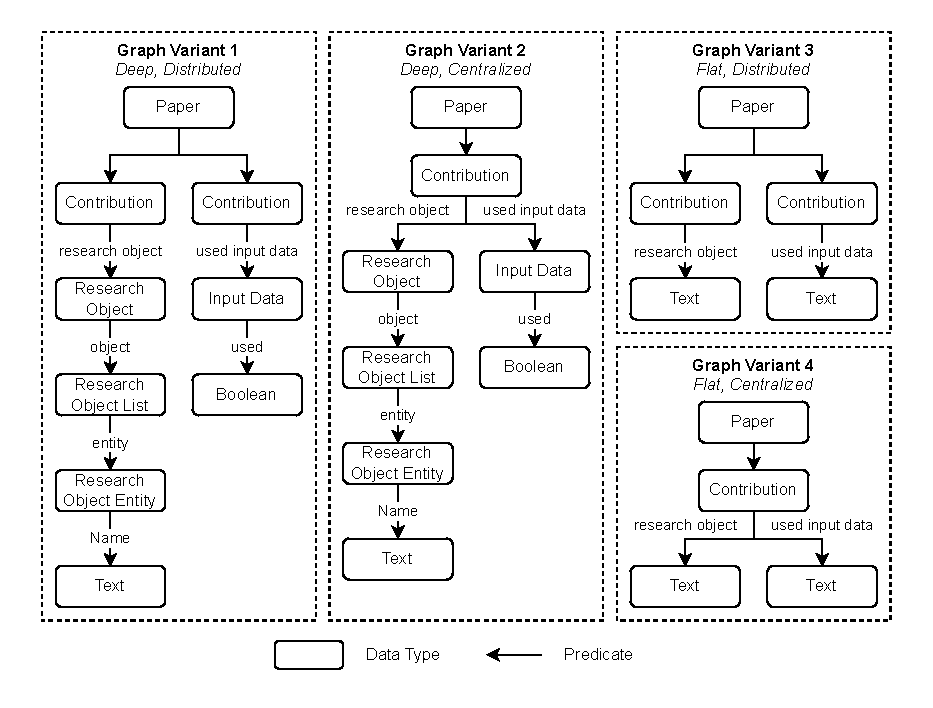
\includegraphics[width=0.93\linewidth]{figures/orkg/template_overview-graph_variants.drawio.pdf}
    \caption[Overview of our Experimentation Graph Templates]{Excerpt of the four different graph variants of the \gls{orkg} featuring the fields research object and input data. This figure highlights the difference between the depth and width of how the same information is stored in each of the different graph variants.}
    \label{fig:overview_graph_variants}
\end{figure}

\begin{enumerate}[leftmargin=2.5em] 
    \item[\textbf{GV1}]\label{enum:gv1} This graph variant stores data in long paths. In addition, the information is semantically separated and distributed between different contributions. 
    \item[\textbf{GV2}]\label{enum:gv2} This graph variant stores data in long paths. All information is collected in a single contribution. 
    \item[\textbf{GV3}]\label{enum:gv3} This graph variant stores data in short paths. The information is semantically separated and distributed across different contributions. 
    \item[\textbf{GV4}]\label{enum:gv4} This graph variant stores data in short paths. All information is collected within a single contribution. 
\end{enumerate}

An illustrative example depicting an excerpt from each of the variants is presented in \autoref{fig:overview_graph_variants}, while the full templates are provided in Appendix~\ref{sec:appendix:orkg_contribution_templates}. The figure shows the root entity of a paper and how information about input data and research objects is stored for each of the four different variants. This highlights the difference in depth and breadth in which the same information is stored between templates.

Using these variants, our aim is to test how robust HubLink is with respect to different graph structures. Long paths allow more information to be stored, but also require more processing. In contrast, short paths limit the amount of stored information, which may result in the loss of semantic context. In addition, we want to examine whether the distribution of data between one or multiple contributions has an effect on performance. Moreover, templates differ in the types that they use to store the data. Consequently, if a \gls{kgqa} approach can be applied to any of the graph variants without requiring a change in its configuration or implementation, it indicates that the approach is \emph{schema-agnostic}. 

The most difficult design decision during the creation of the templates was the multiple classification types in our data. These involve the classification of a paper according to a specific term from a specific selection of terms. For example, whether the paper class is evaluation research, a proposal for a solution, or validation research. To store such information, a typical user interface would provide a \emph{multiple-choice} data type. However, the template system provided by \gls{orkg} does not provide such a datatype at the time of writing. We therefore needed to create such a multiple-choice concept ourselves with the structures provided by the \gls{orkg}. This encompasses several considerations that must be taken into account.

We considered two choices to realize multiple choice. Using \emph{plain text} would allow users to flexibly input their choices. Nevertheless, this approach would not enable the template author to constrain the input, which would be against the idea of consistency in the data, because contribution data types that may relate to the same concept are not guaranteed to have the same value. This includes simple issues like casing, typos, synonyms, etc. Another realization would be a \emph{List of Boolean values}. This would allow the template author to create a list with predefined choices that are relevant. Each choice would be of the type Boolean to determine whether the choice is selected or not. However, the drawback of this approach is that it is less flexible for future extensibility. If the list is later updated to include more choices, all papers that have already used the template will have an empty value for the new choice. However, solving this issue is beyond the scope of this thesis. We implemented both methods in our templates. The variants \textbf{GV1} and \textbf{GV2} implement the list of Boolean, while the variants \textbf{GV3} and \textbf{GV4} store each choice in plain text. The concrete templates for each variant are provided in the Appendix \ref{sec:appendix:orkg_contribution_templates}.

\subsection{Populating the ORKG with Data}
\label{sec:populating_the_orkg}

To store data in the ORKG graph using various templates, a dedicated script was implemented. This script reads the metadata and annotations of the publications from a JSON file and processes each entry iteratively. For each publication, it checks whether it already exists in the graph with all specified contributions. If not, the corresponding contribution is added and populated with the relevant data. The script is triggered automatically whenever the \gls{sqa} system initializes the \gls{orkg} class, which happens before each experiment is run. 

\subsection{Ensuring Repeatability}
\label{sec:orkg_ensuring_repeatability}

During the implementation of the \gls{orkg}, it became evident that inserting data into the graph leads to the automatic generation of unique resource IDs. These IDs cannot be manually controlled and will change if data is deleted and then reinserted into the graph. This poses a challenge since the \gls{kgqa} dataset stores these resource IDs as part of the ground truth to verify whether the correct triples are retrieved during evaluation. If the original data are removed and later reinserted, new resource IDs are generated, which invalidate the \gls{kgqa} datasets.

To address this issue, a script was developed that compares the resource IDs stored in the \gls{kgqa} dataset with the IDs in the graph and updates the IDs in the dataset accordingly. With this approach, we can ensure that the experiments remain reproducible over time. Specifically, this means that the publications can be automatically reinserted into the \gls{orkg} using the \gls{sqa} system in the case that they have been deleted. The system then runs a script that updates the corresponding IDs in the \gls{kgqa} dataset.


\subsection{Reading from the ORKG}
\label{sec:reading_from_the_orkg}

To retrieve data stored in the \gls{orkg}, we use the provided RESTful \gls{api}. This API was integrated into the \gls{sqa} system to enable the automated execution of the experiments. However, during implementation, a key challenge emerged. The \gls{orkg} contains a large amount of data not relevant to our experiments. These additional data introduce noise, making it difficult to establish a controlled experimental setting. Another issue we encountered is that standard users have limited ability to delete data in the \gls{orkg}. This became an issue with our four different graph variants, as the individual deletion of contributions was not possible. Consequently, we stored all variants simultaneously in the graph.

To ensure that an experiment operates only on the data relevant to the experiment, a tailored solution was implemented. During the initialization of the \gls{orkg}, a preprocessing step generates a locally stored list of valid entities and triples. This involves examining all entities and triples in the research field \emph{Software Architecture and Design}, which contains the data relevant to our experiments. Each entity and triple is checked to determine whether they are part of the metadata of a relevant publication or belong to a contribution associated with the currently selected graph variant. Only those triples and entities that meet these criteria are included in the list.

At runtime, this list acts as a filtering mechanism: for each read request made by a retriever, only those triples and entities contained in the prepared list are returned. This ensures that only the intended data for the specific experiment, and exclusively from the selected graph variant, are taken into account.
